\subsection{Handwriting synthesis}
\label{sec:synthesis}

This subsection describes how a text is converted into pen paths in the style of a stored writer (functional units FU~2.7 and part of FU~2.5; requirements R1 and R3).
The synthesiser takes the text, a style profile (Section~\ref{sec:styleprofile}), the x-height size $x_{\mathrm{mm}}$ in millimetres (4\,mm by default) and a random seed, and returns a \emph{trajectory}: pen-down polylines in millimetres, $y$ upwards, origin at the first baseline.
The construction is random, so a search over several candidates (Section~\ref{sec:syn-search}) keeps the one that the text recogniser (Section~\ref{sec:textrec}) and the stroke-normalised writer classifier (Section~\ref{sec:writerid}) jointly prefer.
Geometry stays in x-height units until one multiplication at the end, so one profile serves any pen size.

\subsubsection{Global quantities and glyph choice}

Let $\theta_{\mathrm p}$ be the slant, $c$ the connectedness, $A$ and $D<0$ the ascender and descender reach and $g$ the word gap of the profile, and $\lambda\in[0,1]$ the writer's legibility parameter (below; in the delivered system $\lambda=0$ for every writer, because the key is missing from the stored profiles --- Section~\ref{sec:styleprofile}, so every formula below that contains $\lambda$ should be read at $\lambda=0$ when judging what the submitted code does).
The synthesiser derives, in Equation~\ref{eq:syn-global},
\begin{equation}
\theta_{\mathrm{cap}}=45^\circ-19^\circ\lambda,\quad\sigma=\tan\!\bigl(\operatorname{clip}(\theta_{\mathrm p},\pm\theta_{\mathrm{cap}})\bigr)+\Delta_\sigma,\quad p_{\mathrm j}=\min(c,1),\quad L=(A-D+0.85)\,x_{\mathrm{mm}},
\label{eq:syn-global}
\end{equation}
the shear coefficient $\sigma$ (calibration shift $\Delta_\sigma$, Section~\ref{sec:syn-cal}), the join probability $p_{\mathrm j}$ and the line pitch $L$, which Equation~\ref{eq:syn-global} puts at 12.6\,mm for $A=1.7$, $D=-0.6$ and $x_{\mathrm{mm}}=4$\,mm.
The connectedness is a \emph{probability}: as a threshold it joined every pair for every writer above it and fused words into blobs.

For each character the synthesiser tries, in order, the writer's own variants, a borrowed shape (other case or similar character), the \emph{anchor} glyph, and finally a hand-designed skeleton or a blank.
Variants are ranked by $\mathrm{priorD}$ (Equation~\ref{eq:sty-prior}); only the five best are eligible, and rank $i=0,\ldots,4$ is drawn with probability proportional to the weight of Equation~\ref{eq:syn-pick},
\begin{equation}
w_i=\frac{1}{1+1.4\,i}\exp\!\Bigl[-\Bigl(\frac{\mathrm{entryY}_i-\hat e}{0.45}\Bigr)^2\Bigr],
\label{eq:syn-pick}
\end{equation}
where the exponential factor of Equation~\ref{eq:syn-pick} applies only when the glyph is joined to a previous letter and $\hat e$ is the pen's exit height above the baseline in x-heights: a variant whose entry height matches the pen avoids tangled joins.
Without that exponential factor the five eligible ranks are drawn with probabilities $0.494$, $0.206$, $0.130$, $0.095$ and $0.075$.
A writer forms a letter consistently, and restricting the choice to typical variants gave 80.5\,\% writer identification with the two best variants against 75.5\,\% over all twelve (design-stage measurement, no raw log).

\paragraph{The anchor glyph.}
The \emph{anchor} is a legible stand-in: it is the writer's own medoid if that medoid has $\mathrm{priorD}\le0.30$, and otherwise a hand-designed single-stroke skeleton, joined cursive for $c\ge0.5$ and upright print otherwise, re-proportioned to the writer's reach by $y\mapsto1+(y-1)\max\bigl(0.35,(A-1)/0.75\bigr)$ for $y>1$ and $y\mapsto y\max\bigl(0.35,|D|/0.55\bigr)$ for $y<0$.
The print skeleton reads back at about 96\,\% character and about 84\,\% word accuracy through the recogniser (the figures of the code comment at \texttt{SynthesizeHandwriting.py} line~238, no raw log), which is far clearer than any data-driven consensus glyph, so it is the legibility floor.
\mustdo{the corresponding read-back accuracy of the \emph{cursive} skeleton. An earlier draft of this paragraph quoted about 89\,\% for it; that figure matches no comment or log in the delivered code and has been withdrawn rather than left standing as a measurement.}

\paragraph{The role of $\lambda$.}
The parameter does \emph{not} interpolate geometrically between the writer's glyph and the anchor; it scales the probability, given by Equation~\ref{eq:syn-swap}, that a chosen variant with prior distance $d$ is \emph{replaced} by the anchor,
\begin{equation}
P_{\mathrm{swap}}(\lambda,d)=\begin{cases}1&d\ge0.55,\\0&\lambda\le10^{-3},\\0.06\,\lambda&d\le0.12,\\\operatorname{clip}\bigl(\lambda\,(0.55+0.9\,b),0,1\bigr),\ b=\operatorname{clip}\bigl(\tfrac{d-0.12}{0.43},0,1\bigr)&\text{otherwise,}\end{cases}
\label{eq:syn-swap}
\end{equation}
and it lowers the cap on the writer's own slant (Equation~\ref{eq:syn-global}).
By Equation~\ref{eq:syn-swap} clean glyphs are almost always kept, garbage is always replaced, and in between replacement grows with $\lambda$ (at $\lambda=1$: 0.74 for $d=0.21$, 0.99 for $d=0.33$), so the sources are mixed probabilistically: with the $\lambda$ values of the tuning run the share of anchor glyphs in a design-stage probe ranged from 0\,\% (writer 552, $\lambda=0$) to 76\,\% (writer 151, $\lambda=1$).
$\lambda$ is set per writer (Table~\ref{tab:sty-writers}) by an automatic search on a novel corpus followed by manual adjustment against the evaluation script, so it is tuned on the sentences of Section~\ref{sec:results}.

\emph{Implementation note: in the system as submitted this mechanism is inert.}
The key \texttt{legibilityLambda} is absent from all thirteen stored style profiles, and the entry point the server uses, \texttt{SynthesizeJointBestOf}, defaults the parameter to zero when the key is missing, so $\lambda=0$ for every writer on the live path (Section~\ref{sec:styleprofile}).
The second branch of Equation~\ref{eq:syn-swap} then fires for every glyph whose prior distance is below 0.55, so the \emph{only} anchor substitutions that still happen are the unconditional ones at $d\ge0.55$, and the slant cap of Equation~\ref{eq:syn-global} sits at its widest value $\theta_{\mathrm{cap}}=45^\circ$.
The 0\,\% to 76\,\% range of anchor shares quoted above is therefore the behaviour of the tuned configuration and \emph{not} of the delivered one, where the share is whatever the $d\ge0.55$ rule alone produces; the 76\,\% figure for writer 151 in particular depended on $\lambda=1$ and does not describe the current build.
The $\lambda$ values of Table~\ref{tab:sty-writers} are real measurements of that earlier tuning run and are kept for that reason, labelled as such, and the outstanding item of Section~\ref{sec:styleprofile} to re-run the tuner applies to every $\lambda$-dependent statement in this subsection.
\emph{Further note:} a geometric blend toward the anchor and a ``soft archetype'' proposal appear only in the project notes, not in the delivered code.

\subsubsection{Placement, joins and randomness}

A chosen glyph $(x,y)$ (x-height units, upright) is placed at the pen position $(P_x,P_y)$ (mm) by Equation~\ref{eq:syn-place},
\begin{equation}
X=P_x+(\ell+x+\sigma_g\,y)\,x_{\mathrm{mm}},\qquad Y=P_y+(y+\delta_g)\,x_{\mathrm{mm}},
\label{eq:syn-place}
\end{equation}
with the glyph's lead $\ell$, shear $\sigma_g$ and baseline drift $\delta_g$; Equation~\ref{eq:syn-place} inverts the de-slanting of Equation~\ref{eq:sty-norm}, and Figure~\ref{fig:syn-layout} shows the resulting line-layout geometry.
The writer's own glyphs use $\sigma$; anchor glyphs are limited to $\pm\tan30^\circ$ (cursive) or $\pm\tan22^\circ$ (print), because a $40^\circ$ shear makes even a clean letter collide.
A guard shifts glyph and pen right if the glyph would come closer than $0.05\,x_{\mathrm{mm}}$ to the previous ink, and the pen advances by the glyph's \emph{own} advance, never the character median.
After a word the pen advances by the randomised word gap $g\,x_{\mathrm{mm}}(0.85+0.3u)$ with $u\sim U(0,1)$, and a word that would cross the line width (185\,mm in the server) starts a new line at the pitch $L$.
Adjacent letters are joined if both are alphabetic, both are the writer's own glyphs or both the cursive anchor, and a random $u<p_{\mathrm j}$ (a print anchor is never joined through).
The connector from exit $p_0$ to the next entry $p_1$ is the path of Equation~\ref{eq:syn-lig},
\begin{equation}
\begin{aligned}
&\text{path}(p_0,m,p_1),\qquad m=\Bigl(\tfrac{p_{0x}+p_{1x}}{2},\ \min(p_{0y},p_{1y})-\mathrm{sag}\Bigr),\\
&\mathrm{sag}=\min\bigl(0.11\,x_{\mathrm{mm}},0.16\,|\Delta x|\bigr)+\mathcal N\bigl(0,(0.015\,x_{\mathrm{mm}})^2\bigr),
\end{aligned}
\label{eq:syn-lig}
\end{equation}
with $\Delta x=p_{1x}-p_{0x}$; the sag of Equation~\ref{eq:syn-lig} is proportional to the span because a fixed dip would turn a short join into a loop.
A joined run is one pen-down polyline, so the pen lifts only where the writer lifts, and every polyline is resampled at 0.35\,mm arc length for even plotter motion.
One pseudo-random stream, seeded by the seed argument, supplies every draw, so the arguments fix the output completely.

\begin{figure}[!htbp]
\centering
\begin{tikzpicture}[x=1cm,y=1cm]
\newcommand{\hshape}[1]{\draw[#1] (0.1,0) -- (0.1,1.8); \draw[#1] (0.1,0.6) .. controls (0.3,1.0) and (0.7,1.0) .. (0.75,0.6) -- (0.75,0);}
\draw[gray] (-0.3,0) -- (4.3,0); \node[w3lab,anchor=east] at (-0.3,0) {baseline};
\draw[gray,dashed] (-0.3,1) -- (4.3,1); \node[w3lab,anchor=east] at (-0.3,1) {$y{=}1$};
\begin{scope}[xshift=0.2cm]\hshape{thick}\end{scope}
\begin{scope}[xshift=2.6cm,xslant=0.466]\hshape{thick}\end{scope}
\draw[w3arr] (1.2,0.9) -- (2.2,0.9);
\node[w3lab] at (1.7,1.15) {shear};
\draw[dotted] (2.7,0) -- (2.7,1.8);
\node[font=\scriptsize] at (2.0,-0.45) {(a) $X=\ell+x+y\tan\theta$};
\begin{scope}[xshift=6.3cm]
\draw[gray] (-0.3,0) -- (7.2,0);
\draw[fill=gray!10] (0,0) rectangle (2.3,1.4);
\draw[fill=gray!10] (2.3,0) rectangle (4.3,1.4);
\draw[thick] (0.5,0.1) rectangle (1.9,1.2);
\draw[thick] (2.55,0.1) rectangle (4.0,1.2);
\draw[<->] (0,-0.25) -- (2.3,-0.25); \node[w3lab,anchor=north] at (1.15,-0.25) {advance $a$};
\draw[<->] (0,1.6) -- (0.5,1.6); \node[w3lab,anchor=south] at (0.25,1.6) {$\ell$};
\draw[<->] (1.9,1.6) -- (2.55,1.6); \node[w3lab,anchor=south] at (2.3,1.6) {gap};
\draw[w3arr] (0,-0.9) -- (0.9,-0.9) node[midway,below,w3lab] {$P_x$};
\node[w3lab,anchor=west] at (4.4,0.7) {word gap $g\,x_{\mathrm{mm}}(0.85{+}0.3u)$};
\node[font=\scriptsize] at (3.2,-1.3) {(b) cells, ink boxes and guard};
\end{scope}
\end{tikzpicture}
\caption{Glyph placement. (a) A stored upright glyph is sheared by the writer's slant (Equation~\ref{eq:syn-place}). (b) Each glyph occupies a cell of its own advance $a$; the ink starts after the lead $\ell$, and the collision guard keeps a minimum clear gap between consecutive ink boxes.}
\label{fig:syn-layout}
\end{figure}

\paragraph{Glyph jitter and baseline drift.}
Each glyph receives the random rotation, scaling and translation of amplitude $J$ (0.15 by default, 0.5 in the search) given by Equation~\ref{eq:syn-jit},
\begin{equation}
\begin{pmatrix}x'\\y'\end{pmatrix}=R(\vartheta)\,\mathrm{diag}(s_x,s_y)\begin{pmatrix}x\\y\end{pmatrix}+\begin{pmatrix}d_x\\d_y\end{pmatrix},\quad
\begin{aligned}d_x&\sim\mathcal N(0,(0.022J)^2),&d_y&\sim\mathcal N(0,(0.0132J)^2),\\\vartheta&\sim\mathcal N(0,(2.2^\circ J)^2),&s_{x,y}&\sim1+\mathcal N(0,(0.05J)^2),\end{aligned}
\label{eq:syn-jit}
\end{equation}
with the translations of Equation~\ref{eq:syn-jit} in x-heights; the baseline drifts in addition as a slow first-order walk whose constants are in Table~\ref{tab:syn-const}.
At $J=0.5$ Equation~\ref{eq:syn-jit} gives a translation spread below 0.05\,mm, a rotation of $1.1^\circ$ and a scale change of 2.5\,\%.
Table~\ref{tab:syn-const} collects every remaining constant of the synthesiser and of the jitter model, including those not quoted in the text above.

\begin{table}[!htbp]
\centering
\fontsize{9.5}{11.5}\selectfont
\begin{tabularx}{\linewidth}{|p{5.2cm}|p{2.2cm}|X|}
\hline
\textbf{Constant} & \textbf{Value} & \textbf{Role} \\
\hline
Eligible variants per letter & 5 & Highest-ranked variants that can be drawn (Equation~\ref{eq:syn-pick}). \\
\hline
Clean and garbage prior distances & 0.12 and 0.55 & Limits of Equation~\ref{eq:syn-swap}. \\
\hline
Maximum prior distance of an anchor medoid & 0.30 & Otherwise the generic skeleton is used. \\
\hline
Connected-hand threshold for the cursive anchor & 0.5 & A value above 1 disables the cursive anchor (an earlier configuration used 2.0); lowering it to 0.3 lowered the evaluation score and was reverted. \\
\hline
Slant limit of anchor glyphs & $30^\circ$ / $22^\circ$ & Cursive / print skeleton. \\
\hline
Jitter share of anchor glyphs & 0.15 & Anchor glyphs wobble less. \\
\hline
Collision gap & 0.05 $x_{\mathrm{mm}}$ & Minimum clear space between consecutive ink boxes. \\
\hline
Output resampling and connector step & 0.35\,mm & Arc-length step of every pen-down polyline. \\
\hline
Rendering for the judges & 0.085 $x$, blur 0.30 & Constant pen width in x-heights and Gaussian blur as a fraction of the stroke width; 18 pixels per millimetre; padding $0.18\,x_{\mathrm{mm}}$. \\
\hline
Search stopping scores & 0.99 / 0.995 & Early stop of the candidate loop / no repair above this score. \\
\hline
Repair rounds and pins per round & 3 and 2 & Joint-aware repair pass. \\
\hline
Seed step between candidates & 977 & Candidate $k$ uses $\mathrm{base}+977k$. \\
\hline
Calibration probe & seed 17, $J=0$ & Sentence ``the quick brown fox jumps over lazy dogs and by half past eight it kept flying quietly''. \\
\hline
\end{tabularx}
\begin{tabularx}{\linewidth}{|X|c|c|}
\hline
\textbf{Perturbation (Equation~\ref{eq:syn-jit})} & \textbf{Standard deviation} & \textbf{At $J=0.5$, $x_{\mathrm{mm}}=4$\,mm} \\
\hline
Translation in $x$ / $y$ & $0.022J$ / $0.0132J$ x-heights & 0.044\,mm / 0.026\,mm \\
\hline
Rotation & $2.2^\circ J$ & $1.1^\circ$ \\
\hline
Scale in $x$ and $y$ (independent) & $0.05J$ & 2.5\,\% \\
\hline
Baseline drift (AR(1), clipped) & $0.05J\cdot0.35$ per step, $\pm0.25$ & $\pm0.25$ x-heights \\
\hline
Connector sag noise & $0.015\,x_{\mathrm{mm}}$ & 0.06\,mm \\
\hline
Word-gap factor & uniform 0.85 to 1.15 & --- \\
\hline
\end{tabularx}
\caption{Constants of the synthesiser and the jitter model.}
\label{tab:syn-const}
\end{table}

\paragraph{Style calibration.}
\label{sec:syn-cal}
A line of separate glyphs does not automatically reproduce the line-level slant and reach of the real lines (writer 150's ascenders came out about 7\,\% too tall, writer 551's slant about $9^\circ$ too steep).
A probe sentence is therefore synthesised once per writer and size, measured with the estimators of Section~\ref{sec:styleprofile}, and three fixed-point iterations adjust the shear shift $\Delta_\sigma$ and the scale factors $K_A$, $K_D$ of the writer's own tall and deep strokes until the probe matches the stored real-line values.
Writing ``ref'' for the stored real-line value and ``got'' for the value measured on the probe, the three iterations are those of Equation~\ref{eq:syn-cal},
\begin{equation}
\Delta_\sigma\leftarrow\Delta_\sigma+\tan\theta_{\mathrm{ref}}-\tan\theta_{\mathrm{got}},\quad K_A\leftarrow\operatorname{clip}\Bigl(K_A\frac{A_{\mathrm{ref}}-1}{A_{\mathrm{got}}-1},0.5,1.6\Bigr),\quad K_D\leftarrow\operatorname{clip}\Bigl(K_D\frac{D_{\mathrm{ref}}}{D_{\mathrm{got}}},0.5,1.6\Bigr),
\label{eq:syn-cal}
\end{equation}
in which $\theta$ is the line slant of Equation~\ref{eq:sty-slant}, $A>1$ the ascender reach and $D<0$ the descender reach, the stored reference values being \texttt{slantMeasRef}, \texttt{ascMeasRef} and \texttt{descMeasRef} of Table~\ref{tab:sty-schema}.
The scale factors of Equation~\ref{eq:syn-cal} are applied as $y\leftarrow1+(y-1)K_A$ for $y>1$ and $y\leftarrow yK_D$ for $y<0$ on the writer's own glyphs, the clip to $[0.5,1.6]$ bounding the correction, and $\Delta_\sigma$ is added to the shear coefficient of Equation~\ref{eq:syn-global}.
The probe is synthesised with seed 17 and no jitter (Table~\ref{tab:syn-const}).
The same estimator measures both sides, so the agreement of slant and reach is partly self-fulfilling and not independent evidence.

\subsubsection{Best-of-$N$ search with joint scoring}
\label{sec:syn-search}

Single draws vary in quality, so the line is drawn $N$ times and the best candidate kept.
Selecting by text accuracy alone raised legibility but lowered writer identification for some writers (Table~\ref{tab:syn-evid}): the most legible draw need not be the most characteristic.
The score therefore uses both judges.
For a rendered candidate $I$, with $\hat y(I)$ the greedy CTC reading (Equation~\ref{eq:rec-greedy}) and $y$ the intended text, the joint score is given by Equation~\ref{eq:syn-score},
\begin{equation}
a(I)=\max\Bigl(0,1-\frac{\mathrm{Lev}(\hat y(I),y)}{|y|}\Bigr),\quad w(I)=\mathrm{softmax}\bigl(f_{\mathrm{wid}}(I)\bigr)_{a^\star},\quad S(I)=\frac{2\,a(I)\,w(I)}{a(I)+w(I)},
\label{eq:syn-score}
\end{equation}
where in Equation~\ref{eq:syn-score} $\mathrm{Lev}$ is the Levenshtein distance (Equation~\ref{eq:rec-lev}), $f_{\mathrm{wid}}$ the shape classifier after stroke normalisation (Section~\ref{sec:wid-strokenorm}), $a^\star$ the target writer, and $S=0$ if $a+w\le10^{-9}$.
The harmonic mean is dominated by the smaller term, so a candidate cannot win on one criterion while failing the other, and $w$ is a probability, not a hit-or-miss flag.

\paragraph{Steps of the search and the repair pass.}
The steps of Figure~\ref{fig:syn-flow} are:
(1) for $k=0,\ldots,N-1$, synthesise a candidate with seed $\mathrm{base}+977k$ and $J=0.5$, render it at a constant pen width of 0.085 x-heights (18 pixels per millimetre), compute $S$ (Equation~\ref{eq:syn-score}), keep it if $S>\mathrm{best}$ (initially $-1$), and stop early at $\mathrm{best}\ge0.99$;
(2) \emph{repair} (at most three rounds, skipped if $\mathrm{best}\ge0.995$): forced-align the intended text to the recogniser output on the best image (Equation~\ref{eq:sty-viterbi}) and score each non-space character $i$ by its mean own-class log-probability over its frames, Equation~\ref{eq:syn-weak},
\begin{equation}
m_i=\frac{1}{b_i-a_i}\sum_{t=a_i+1}^{b_i}\ell_t(y_i),
\label{eq:syn-weak}
\end{equation}
where Equation~\ref{eq:syn-weak} is set to $m_i=-10^9$ if the path never visits character $i$, and the characters are sorted ascending by $m_i$;
(3) pin the two worst unpinned characters to the anchor, re-synthesise the \emph{whole} line with seed $\mathrm{base}$, render and score it;
(4) accept only if the joint score strictly exceeds $\mathrm{best}$.
A repaired line is therefore accepted only if the joint score strictly exceeds the best so far, so a repair that fixes a letter but makes the line look like another writer is rejected (a text-only search with a plain repair that accepts on text score alone was measured to cost writer identification; Table~\ref{tab:syn-evid}).

\begin{figure}[!htbp]
\centering
\begin{tikzpicture}[x=1cm,y=1cm]
\tikzset{n/.style={w3box,text width=3.6cm,minimum height=0.7cm,font=\scriptsize},d/.style={w3dec,text width=2.1cm}}
\node[w3io,text width=3.6cm,font=\scriptsize,minimum height=0.7cm] (s0) at (0,0) {Text, writer, $N$, base seed};
\node[n] (s1) at (0,-1.0) {Synthesise candidate $k$, seed $\mathrm{base}+977k$, $J=0.5$};
\node[n] (s2) at (0,-2.0) {Render at constant pen width};
\node[n] (s3) at (0,-3.0) {Judges $a(I)$, $w(I)$; $S(I)$ (Eq.~\ref{eq:syn-score})};
\node[d] (s4) at (0,-4.2) {$S>\mathrm{best}$?};
\node[d] (s5) at (0,-5.7) {$\mathrm{best}\ge0.99$ or $k=N-1$?};
\node[n,text width=2.0cm] (keep) at (3.0,-4.2) {keep candidate};
\node[n] (r1) at (7.0,-0.3) {Forced-align text; rank characters by $m_i$ (Eq.~\ref{eq:syn-weak})};
\node[d] (r0) at (7.0,-1.6) {$\mathrm{best}\ge0.995$ or 3 rounds?};
\node[n] (r2) at (7.0,-2.9) {Pin the 2 worst unpinned characters to the anchor};
\node[n] (r3) at (7.0,-3.9) {Re-synthesise line, seed $=\mathrm{base}$; judge};
\node[d] (r4) at (7.0,-5.0) {$S'>\mathrm{best}$?};
\node[n,text width=2.2cm] (acc) at (10.0,-5.0) {accept; keep pins};
\node[w3io,text width=3.0cm,font=\scriptsize,minimum height=0.7cm] (out) at (7.0,-6.3) {Trajectory to G-code};
\draw[w3arr] (s0) -- (s1); \draw[w3arr] (s1) -- (s2); \draw[w3arr] (s2) -- (s3); \draw[w3arr] (s3) -- (s4);
\draw[w3arr] (s4) -- (keep) node[midway,above,w3lab] {yes};
\draw[w3arr] (s4) -- (s5) node[midway,right,w3lab] {no};
\draw[w3arr] (keep.south) |- (s5.east);
\draw[w3arr] (s5.west) -- ++(-1.6,0) |- (s1.west) node[pos=0.2,left,w3lab] {no};
\draw[w3arr] (s5.south) -- ++(0,-0.45) -| ++(3.6,0) |- (r1.west) node[pos=0.1,right,w3lab] {yes};
\draw[w3arr] (r1) -- (r0);
\draw[w3arr] (r0) -- (r2) node[midway,right,w3lab] {no};
\draw[w3arr] (r2) -- (r3); \draw[w3arr] (r3) -- (r4);
\draw[w3arr] (r4) -- (acc) node[midway,above,w3lab] {yes};
\draw[w3arr] (r4.south) -- (out.north) node[pos=0.3,right,w3lab] {no};
\draw[w3arr] (acc.south) |- (out.east);
\draw[w3arr] (r0.east) -- ++(1.3,0) |- ++(0,-4.4) |- (out.east);
\end{tikzpicture}
\caption{Flow chart of the joint best-of-$N$ search: the search over $N$ candidates (left) and the repair pass (right). A repair round ends after acceptance or rejection and the next round starts from the best candidate; when its test is satisfied the repair loop exits to the output.}
\label{fig:syn-flow}
\end{figure}

If candidate scores were independent with distribution function $F$, then the order statistic of Equation~\ref{eq:syn-order},
\begin{equation}
\Pr\bigl[\max_kS_k\le\tau\bigr]=F(\tau)^N,
\label{eq:syn-order}
\end{equation}
shows that the gain of Equation~\ref{eq:syn-order} grows roughly logarithmically in $N$; the seeds share a profile, so independence is only approximate, and no per-$N$ curve was kept.
\emph{Implementation notes.} (i) The repair re-uses seed $\mathrm{base}$, so it is a fresh draw with pins, not a patch of the winner. (ii) The pin set is updated only on acceptance, so after a rejection the next round re-synthesises an identical candidate and the remaining rounds are wasted work. (iii) In three probe runs (writers 150, 153, 551, $N=14$) no repair was accepted, so the repair pass rarely changes the result.

\paragraph{Values of $N$ and cost.}
$N$ is 6 as the function default, 14 for the design-stage measurements of Table~\ref{tab:syn-evid}, 20 as the web default and 30 in the official evaluation script.
A candidate costs one synthesis, one rendering, one recogniser pass and one classifier pass, so the total cost is that of Equation~\ref{eq:syn-cost},
\begin{equation}
T\approx N\,(T_{\mathrm{syn}}+T_{\mathrm{ren}}+T_{\mathrm{text}}+T_{\mathrm{wid}})+\text{(up to three repair candidates)},
\label{eq:syn-cost}
\end{equation}
and each network pass in Equation~\ref{eq:syn-cost} is about $4\times10^9$ multiply--accumulate operations (Equation~\ref{eq:rec-macs}, Table~\ref{tab:wid-layers}).
Laptop timings per stage are in Table~\ref{tab:syn-cost}: synthesis takes 11 to 16\,ms per candidate and the two judges 0.5 to 4\,s, dominated by thinning the full-resolution render, so the search at $N=14$ took 23 to 137\,s; times on the single-board computer were not recorded.

\begin{table}[!htbp]
\centering
\fontsize{9.5}{11.5}\selectfont
\begin{tabularx}{\linewidth}{|X|c|c|c|}
\hline
\textbf{Quantity (56-character sentence)} & \textbf{Writer 150} & \textbf{Writer 153} & \textbf{Writer 551} \\
\hline
Render size (pixels) & $3585\times225$ & $5508\times207$ & $7876\times277$ \\
\hline
Synthesis of one candidate (ms) & 11 & 13 & 16 \\
\hline
Rendering (ms) & 20 & 27 & 56 \\
\hline
Text recogniser (s) & 0.50 & 0.49 & 0.74 \\
\hline
Writer classifier incl. stroke normalisation (s) & 1.03 & 1.65 & 3.74 \\
\hline
Complete search, $N=14$, with repair attempts (s) & 23 & 37 & 137 \\
\hline
\end{tabularx}
\caption{Indicative cost of the search on the development laptop (single profiling run, unknown background load, jitter 0.5); times on the single-board computer were not recorded.}
\label{tab:syn-cost}
\end{table}

\subsubsection{Design-stage measurements of the synthesiser}

Table~\ref{tab:syn-evid} lists the measurements that motivated the design (six novel sentences, two seeds, ten writers: 12 lines per writer, so one misjudged line moves a writer's rate by 8.3 percentage points), together with the final system for comparison.
\emph{Every figure after the search was introduced is the opinion of the very networks that selected the output}: the search loads the same weight files as the measurement, so a selection effect is added to genuine quality, and $\lambda$, the anchor threshold and $N$ were tuned on the same sentences.
The values show that the pipeline can satisfy these two judges, not that human readers or an independent recogniser agree; the non-circular reference is the recogniser on \emph{real} held-out handwriting of the same writers, 89.4\,\% character and 70.8\,\% word accuracy (Table~\ref{tab:rec-data}; possible training overlap).
Section~\ref{sec:results} reports the final evaluation.

\begin{table}[!htbp]
\centering
\fontsize{9.5}{11.5}\selectfont
\begin{tabularx}{\linewidth}{|X|c|c|}
\hline
\textbf{Stage} & \textbf{Writer ID, direct / G-code (\%)} & \textbf{Char. acc., direct / G-code (\%)} \\
\hline
Plain synthesis after label and glyph fixes & 79.2 / 80.0 & 75.9 / 76.3 \\
\hline
+ per-writer $\lambda$ & 83.3 / 86.7 & 77.2 / 77.8 \\
\hline
Text-only best-of-$N$ with plain repair & 76.7 / 73.3 & 83.8 / 82.7 \\
\hline
Joint best-of-$N$, $N=6$ & 92.5 / 92.5 & 79.9 / 79.6 \\
\hline
Joint best-of-$N$, $N=14$ & 97.5 / 95.8 & 81.6 / 81.4 \\
\hline
\textbf{Final system, 13 writers, 3 sentences, $N=8$} & \textbf{92.3 / 89.7} & \textbf{79.2 / 79.2} \\
\hline
\textbf{Final system, 13 writers, 6 sentences $\times$ 2 seeds, $N=30$} & \textbf{80.1 / 78.8} & \textbf{82.2 / 82.5} \\
\hline
\textbf{Matching comparison: the writers' own handwriting of the same words} & not applicable & \textbf{89.0 / ---} \\
\hline
\textbf{Matching comparison: the system's synthesis of those same words} & not applicable & \textbf{81.6 / ---} \\
\hline
\end{tabularx}
\caption{Measurements that motivated the design (upper rows) and the final system (lower rows). ``G-code'' means converted to G-code and read back (Section~\ref{sec:gcode}). The upper rows and the writer-identification columns are judged by the networks that drive the search and were tuned on the same sentences, so they are not independent evidence; the two matching-comparison rows are independent of the search and are the figures to trust. The gain shown in the ``per-writer $\lambda$'' row is not available in the delivered system: the key \texttt{legibilityLambda} is absent from the stored profiles, so the live path runs at $\lambda=0$ (Section~\ref{sec:styleprofile}).}
\label{tab:syn-evid}
\end{table}

Four remarks follow from Table~\ref{tab:syn-evid}.
First, on the matching comparison of identical words the writers' own hands are read at 89.0\,\% and the synthesis of those words at 81.6\,\% character accuracy, so synthesis costs 7.4 percentage points.
Second, the same comparison divides word accuracy by more than 1.5 (70.5\,\% against 46.7\,\%), locating the loss in spacing and word boundaries rather than letterforms.
Third, at the final settings the two most joined writers stay well below the 85\,\% target: writers 151 and 552 reach 53\,\% and 56\,\% character accuracy through G-code, against about 84\,\% for the other eleven.
This is the clearest limitation of the exemplar approach on strongly cursive hands.
Fourth, the writer-identification figures on synthesised text (80.1\,\% in the official run and 89.7\,\% in the coverage run) come from a classifier that also selects the candidates, so a best-of-$N$ search necessarily raises the score by which it is judged; they are reported as what the system computes at run time, not as an independent measure of style.
For these reasons the measurements of Table~\ref{tab:syn-evid} motivated the settings of this block but cannot stand as a verification of it.
Figure~\ref{fig:res-e2e} shows the per-writer breakdown and Figure~\ref{fig:syn-lines} one candidate each for a print and a joined hand.

\begin{figure}[!htbp]
\centering

\includegraphics[width=\linewidth]{Figures/w3_synth_150.png}\\[2pt]
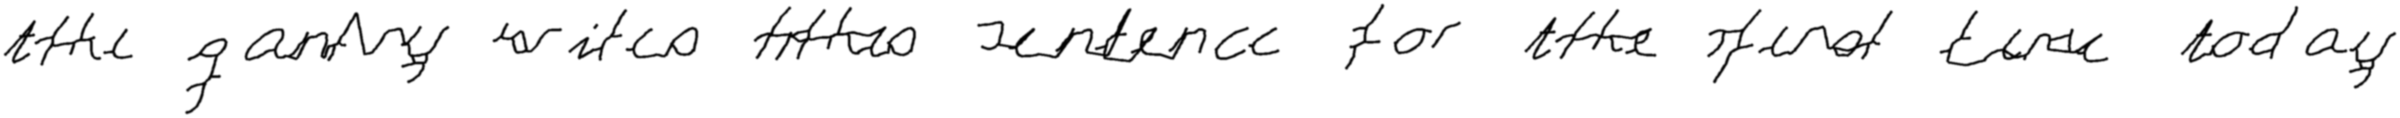
\includegraphics[width=\linewidth]{Figures/w3_synth_153.png}
\caption{Synthesised line ``The gantry writes this sentence for the first time today'' for writer 150 (upper, printed hand; read back with three small errors) and writer 153 (lower, joined hand; read back as ``the garoby writes tttas senkence for tthe furst tuse today''), one seed and candidate each, rendered from the trajectory of an end-to-end run; the $N$ of that run was not recorded.}
\label{fig:syn-lines}
\end{figure}

\subsubsection{Design alternatives and justification}

Table~\ref{tab:syn-alt} lists the alternatives with the assessment of each.
A recurrent sequence generator with attention and mixture-density output~\cite{graves2013} needs on-line pen data (hundreds to thousands of lines per writer), whereas only 47 to 130 scanned lines per writer exist (Table~\ref{tab:sty-writers}); a from-scratch version trained on skeleton-derived strokes learned slant, roundness and connectedness but no legible letters and was rejected.
Adversarial and diffusion generators of line images~\cite{kang2020,dai2024} need less data, but their output is a raster needing the same thinning to vectorise, size, slant and spacing cannot be controlled, and a trial took 35 to 45\,s per line on a laptop processor against 3 to 8\,s for glyph synthesis.
The glyph library needs about nine pages per writer and no training, outputs pen strokes directly, exposes size, slant, joins and gap as numbers, traces a failure to a single glyph and has a fallback for every glyph; its weakness is joined hands, whose joins are lost by cutting.
Glyph assembly from one writer's sample~\cite{haines2016} is a related approach.
Synthesis costs about 15\,ms, so only the optional search is expensive, suiting a single-board computer without accelerator.

\begin{table}[!htbp]
\centering
\fontsize{9.5}{11.5}\selectfont
\begin{tabularx}{\linewidth}{|p{3.2cm}|X|}
\hline
\textbf{Alternative} & \textbf{Assessment} \\
\hline
Recurrent sequence generator with attention and mixture-density output~\cite{graves2013} & Natural cursive, but needs on-line pen data (hundreds to thousands of lines per writer); only 47 to 130 scanned lines per writer exist. A from-scratch version trained on skeleton-derived strokes learned slant, roundness and connectedness but no legible letters. Rejected. \\
\hline
Adversarial or diffusion image generators~\cite{kang2020,dai2024} & Low data need through pre-training, but the output is a raster: it needs vectorisation with the same thinning artefacts, size, slant and spacing cannot be controlled, and a trial took 35 to 45\,s (one line, laptop processor) to 2--3\,min against 3 to 8\,s for glyph synthesis. Rejected and parked. \\
\hline
Glyph assembly from one writer's sample~\cite{haines2016} & Related approach; the present design adds the recogniser-aligned profile and the judge-driven search. \\
\hline
Glyph library with search (chosen) & Needs about nine pages per writer and no training; pen strokes are the native output; size, slant, joins and gap are explicit numbers; failures trace to one glyph; every glyph has a fallback. Weakness: cursive hands, whose joins are lost by cutting. \\
\hline
\end{tabularx}
\caption{Alternatives to the glyph-library synthesiser (timings are trial runs on a laptop without accelerator).}
\label{tab:syn-alt}
\end{table}
